%%%%%%%%%%%%%%%%%%%%%%%%%%%%%%%%%%%%%%%%%%%%%%%%%%%%%%%%%%%%%%%%%%%%%%%%%%%%%%%%
% USENIX Security 2027 submission draft.
% The official USENIX style is vendored as usenix.sty.
% Test-set numbers are generated from immutable run artifacts.
%%%%%%%%%%%%%%%%%%%%%%%%%%%%%%%%%%%%%%%%%%%%%%%%%%%%%%%%%%%%%%%%%%%%%%%%%%%%%%%%
\documentclass[letterpaper,twocolumn,10pt]{article}
% Tectonic uses XeTeX; preload hyperref because the official USENIX style
% loads breakurl before hyperref, which breakurl rejects under XeTeX.
\usepackage{hyperref}
\usepackage{usenix}
\usepackage{amsmath,amssymb}
\usepackage{booktabs}
\usepackage{graphicx}
\usepackage{multirow}
\usepackage{xspace}
\usepackage{xurl}

\newcommand{\system}{\textsc{WarrantLab}\xspace}
\newcommand{\udcr}{\textsc{UDCR}\xspace}
\newcommand{\todoresult}{\textnormal{--}}

% This file is regenerated from analysis.json and statistics.json.  Fallbacks
% keep the source compilable while a frozen run is still in progress.
\IfFileExists{generated_results.tex}{% Generated; do not edit by hand.
% run_id=test-canonical-remote-fusion-gemma-v1_4-r3
% analysis_sha256=01990646960e343adc03de462c54fb7f37dee326004009ed53badf52d5a86da3
% statistics_sha256=12cf5ae1ed061391e323709c2f66d717b5ec5275ab054b71a0ed8cb3d9b34d8e
% records_sha256=6975c933def631c6a5f4095bb995f3948a5ced0c25da98b347a73c945af6e007
\newcommand{\TestRecords}{540}
\newcommand{\TestBaseCases}{36}
\newcommand{\TestVariants}{1}
\newcommand{\OperationalValidity}{99.1\%}
\newcommand{\AlertsAccuracy}{94.4\%}
\newcommand{\AlertsCoverage}{94.4\%}
\newcommand{\AlertsAttackRecall}{98.1\%}
\newcommand{\AlertsBenignRejection}{90.7\%}
\newcommand{\AlertsUnsafeExposure}{.667}
\newcommand{\AlertsRawUDCR}{26.2\%}
\newcommand{\AlertsCitationValidity}{100.0\%}
\newcommand{\EventsAccuracy}{91.7\%}
\newcommand{\EventsCoverage}{91.7\%}
\newcommand{\EventsAttackRecall}{100.0\%}
\newcommand{\EventsBenignRejection}{83.3\%}
\newcommand{\EventsUnsafeExposure}{.444}
\newcommand{\SelfAccuracy}{44.4\%}
\newcommand{\SelfCoverage}{44.4\%}
\newcommand{\SelfAttackRecall}{64.8\%}
\newcommand{\SelfUnsafeExposure}{.333}
\newcommand{\VerifierAccuracy}{85.2\%}
\newcommand{\VerifierCoverage}{85.2\%}
\newcommand{\VerifierAttackRecall}{81.5\%}
\newcommand{\VerifierUnsafeExposure}{.667}
\newcommand{\AbstainAccuracy}{45.4\%}
\newcommand{\AbstainCoverage}{45.4\%}
\newcommand{\AbstainAttackRecall}{57.4\%}
\newcommand{\AbstainBenignRejection}{33.3\%}
\newcommand{\AbstainUnsafeExposure}{.000}
\newcommand{\AbstainDeliveredUDCR}{0.0\%}
\newcommand{\UnsafeDifference}{-.667}
\newcommand{\UnsafeCILow}{-.981}
\newcommand{\UnsafeCIHigh}{-.380}
\newcommand{\RecallDifference}{-.407}
\newcommand{\RecallCILow}{-.630}
\newcommand{\RecallCIHigh}{-.185}
\newcommand{\CoverageDifference}{-.491}
\newcommand{\CoverageCILow}{-.648}
\newcommand{\CoverageCIHigh}{-.333}
\newcommand{\NoninferiorResult}{not}
\newcommand{\AlertVerdictFlip}{9.3\%}
\newcommand{\AlertActorFlip}{0.0\%}
}{
  \newcommand{\TestRecords}{\todoresult}
  \newcommand{\TestBaseCases}{36}
  \newcommand{\TestVariants}{\todoresult}
  \newcommand{\OperationalValidity}{\todoresult}
  \newcommand{\AlertsAccuracy}{\todoresult}
  \newcommand{\AlertsCoverage}{\todoresult}
  \newcommand{\AlertsAttackRecall}{\todoresult}
  \newcommand{\AlertsBenignRejection}{\todoresult}
  \newcommand{\AlertsUnsafeExposure}{\todoresult}
  \newcommand{\AlertsRawUDCR}{\todoresult}
  \newcommand{\AlertsCitationValidity}{\todoresult}
  \newcommand{\EventsAccuracy}{\todoresult}
  \newcommand{\EventsCoverage}{\todoresult}
  \newcommand{\EventsAttackRecall}{\todoresult}
  \newcommand{\EventsBenignRejection}{\todoresult}
  \newcommand{\EventsUnsafeExposure}{\todoresult}
  \newcommand{\SelfAccuracy}{\todoresult}
  \newcommand{\SelfCoverage}{\todoresult}
  \newcommand{\SelfAttackRecall}{\todoresult}
  \newcommand{\SelfUnsafeExposure}{\todoresult}
  \newcommand{\VerifierAccuracy}{\todoresult}
  \newcommand{\VerifierCoverage}{\todoresult}
  \newcommand{\VerifierAttackRecall}{\todoresult}
  \newcommand{\VerifierUnsafeExposure}{\todoresult}
  \newcommand{\AbstainAccuracy}{\todoresult}
  \newcommand{\AbstainCoverage}{\todoresult}
  \newcommand{\AbstainAttackRecall}{\todoresult}
  \newcommand{\AbstainBenignRejection}{\todoresult}
  \newcommand{\AbstainUnsafeExposure}{\todoresult}
  \newcommand{\AbstainDeliveredUDCR}{\todoresult}
  \newcommand{\UnsafeDifference}{\todoresult}
  \newcommand{\UnsafeCILow}{\todoresult}
  \newcommand{\UnsafeCIHigh}{\todoresult}
  \newcommand{\RecallDifference}{\todoresult}
  \newcommand{\RecallCILow}{\todoresult}
  \newcommand{\RecallCIHigh}{\todoresult}
  \newcommand{\CoverageDifference}{\todoresult}
  \newcommand{\CoverageCILow}{\todoresult}
  \newcommand{\CoverageCIHigh}{\todoresult}
  \newcommand{\NoninferiorResult}{\todoresult}
  \newcommand{\AlertVerdictFlip}{\todoresult}
  \newcommand{\AlertActorFlip}{\todoresult}
}

\date{}
\title{\Large \bf Citations Are Not Grounding:\\
Measuring Evidential Warrant in LLM Cloud Forensics}

% USENIX Security uses double-blind review.  Restore authors only after review.
\author{{\rm Anonymous submission}}

\begin{document}
\maketitle

\begin{abstract}
Large language models increasingly produce incident reports whose claims cite
real log records.  A resolvable citation, however, can be relevant without
licensing the reported actor, intent, causal chain, or final accusation.  We
call this discrepancy the \emph{forensic warrant gap}.  We introduce
\system, an evaluation method that decomposes an investigation into atomic
claims and scores citation, actor, action, object, time, quantity, scope,
modality, authorization, intent, causality, and decision strength separately.
Its benchmark contains 48 independently parameterized cases from 12 cloud
incident families, each rendered into ten paired evidence and context
mutations (480 records).  We compare events-only generation, alert-conditioned
generation, self-review, alert-blind verification, and verification followed
by abstention; stochastic conditions use three repetitions and inference is
clustered by base case.  In the frozen held-out evaluation, alert-conditioned
generation surfaced \AlertsUnsafeExposure\ unwarranted decisive claims per
case at \AlertsCoverage\ coverage.  Verification plus abstention changed this
exposure by \UnsafeDifference\ (95\% cluster-bootstrap CI
[\UnsafeCILow,~\UnsafeCIHigh]) but changed attack recall by
\RecallDifference\ [\RecallCILow,~\RecallCIHigh] and coverage by
\CoverageDifference\ [\CoverageCILow,~\CoverageCIHigh].  Thus, the safety
gain did \NoninferiorResult\ satisfy the pre-specified 3-point recall
non-inferiority margin.  Citation validity remained
\AlertsCitationValidity---showing why it is an inadequate safety metric.  The
study supports atomic warrant evaluation and selective reporting, but not
autonomous forensic attribution; the principal result is a measurable safety--
coverage trade-off rather than a detector-accuracy claim.
\end{abstract}

%-------------------------------------------------------------------------------
\section{Introduction}
\label{sec:introduction}
%-------------------------------------------------------------------------------

An investigator receives an alert naming an employee, inspects a set of cloud
logs, and asks a large language model (LLM) to reconstruct the incident.  The
model returns a polished report: every sentence cites an event identifier, and
every identifier resolves.  This output looks auditable.  Yet the cited login
may establish only that an account authenticated, not who controlled it; a
transfer record may establish bytes sent, not theft; events adjacent in time
may not form a causal chain; and an alert may merely repeat the very hypothesis
the investigation is supposed to test.  A citation can therefore be valid
while the attached claim is too strong.

This distinction matters in digital forensics.  Wrong-actor attribution can
harm an employee, a false causal story can redirect containment, and a fluent
``confirmed incident'' can be mistaken for a conclusion rather than a
hypothesis.  Existing evidence-grounded generation work separates citation
correctness and completeness~\cite{gao2023alce,min2023factscore}; recent
evidence-force work shows that even relevant citations may under-warrant a
claim's modality, scope, time, or number~\cite{qian2026forcebench}.  Security
systems, meanwhile, increasingly combine LLM reasoning with alerts, tools, and
retrieved logs~\cite{loumachi2025gendfir,wei2025cortex,cadet2026rag}.  Their
evaluation usually emphasizes final verdicts or answer quality.  It rarely
asks, proposition by proposition, whether visible evidence licenses the exact
forensic language that reaches an analyst.

We study that missing unit of evaluation.  An \emph{atomic forensic claim}
contains one subject--predicate--object assertion plus explicit qualifiers,
cited event identifiers, confidence, materiality, and claimed evidence
relation.  \emph{Evidential warrant} requires the cited evidence to license
every material field; an existing or topically related event is insufficient.
This definition turns an investigation from an indivisible narrative into an
auditable set of propositions.

We instantiate the definition in \system, a benchmark, output contract,
conservative evaluator, blinded annotation workflow, and paired intervention.
The 480-record synthetic benchmark crosses 48 independent base cases, 12
attack and legitimate-but-suspicious families, and ten mutations.  Mutations
hold core evidence fixed while changing alert actor/severity, adding decoys or
irrelevant noise, withholding decisive or exculpatory evidence, drifting the
schema, or inserting passive prompt injection.  Crucially, the benchmark
separates the incident that occurred from the verdict warranted by the
\emph{visible} record.  Evidence removal can therefore make
\textsc{insufficient} the only responsible answer even when the latent
scenario contains an attack.

Our intervention uses one alert-visible generator response for all downstream
review conditions.  Self-review or an independent alert-blind verifier may
recommend abstention; a deterministic policy then withholds outputs containing
unsupported decisive claims or unresolved decisive counterevidence.  Sharing
the exact generator response isolates review from sampling variation.

The paper makes four contributions:

\begin{itemize}
  \item We define a forensic warrant ontology spanning citation, actor,
  action, object, time, quantity, scope, modality, authorization, intent,
  causality, and decision strength, together with a machine-checkable atomic
  claim contract.
  \item We release a paired 480-record benchmark with hidden/visible ground
  truth, provenance-tagged mutations, base-case-disjoint development and test
  splits, deterministic baselines, and attack-bearing untrusted log content.
  \item We give a paired evaluation of alert context, self-review,
  independent verification, and abstention.  It reports unsafe claim exposure
  jointly with coverage and recall, preventing an always-abstain system from
  appearing safe.
  \item We provide a reproducible protocol: frozen prompts and schemas, raw
  response hashes, append-only failures, base-case cluster bootstrap,
  prevalence-adjusted operating points, and a blinded two-annotator package.
\end{itemize}

The result is deliberately bounded.  The benchmark is synthetic, one remote
deployment exposes only a model alias, and expert labels are required before
the mechanical warrant proxy can support a forensic-validity claim.  These are
not footnotes to conceal; they define what the study can and cannot establish.

%-------------------------------------------------------------------------------
\section{The Forensic Warrant Gap}
\label{sec:warrant-gap}
%-------------------------------------------------------------------------------

\subsection{Four properties often called grounding}

We separate four nested properties:

\begin{enumerate}
  \item \textbf{Citation validity:} each cited identifier resolves to a
  visible event.
  \item \textbf{Citation completeness:} every material claim cites its
  purported evidence.
  \item \textbf{Evidential warrant:} the cited events license the exact
  material fields and strength of the claim.
  \item \textbf{Decision reliability:} the final verdict and attribution are
  correct, calibrated, robust to irrelevant context, and able to abstain.
\end{enumerate}

The first two are surface properties.  A report can score perfectly on both
while failing the latter two.  This is the forensic analogue of citation
laundering: a real event lends visual authority to a conclusion it does not
establish~\cite{qian2026forcebench}.

\subsection{Atomic claim contract}

An investigation output $O$ contains verdict $v\in\{\textsc{yes},
\textsc{no},\textsc{insufficient}\}$, optional suspect $s$, evidence for and
against the leading hypothesis, missing evidence, alternatives, overall
confidence, and claims $C=\{c_1,\ldots,c_m\}$.  Each claim is

\begin{equation}
c_i=(t_i,a_i,p_i,o_i,\tau_i,q_i,M_i,A_i,I_i,E_i,r_i,d_i,\gamma_i),
\end{equation}

where $t$ is claim type; $a,p,o$ are actor, predicate, and object; $\tau$ is
time; $q$ is quantity; $M$ is modality; $A$ is authorization; $I$ is intent;
$E$ is a set of cited event identifiers; $r$ is the claimed relation
(supports, contradicts, or insufficient); $d$ marks decisiveness; and
$\gamma\in[0,1]$ is confidence.  Optional scope and causal-parent fields are
also explicit.  Free-form prose is a rendering of this record, not the
authoritative object.

For axis $k$, evaluator $g_k(c_i,E)$ returns \textsc{supported},
\textsc{contradicted}, \textsc{insufficient}, or \textsc{not-applicable}.  A
material claim is warranted only when every applicable material axis is
supported:

\begin{equation}
W(c_i,E)=\mathbb{1}\!\left[\forall k\in K_i,
g_k(c_i,E)=\textsc{supported}\right].
\end{equation}

This conjunction is intentionally strict.  Correct actor and action fields do
not rescue an unsupported causal link or ``confirmed'' modality.

\subsection{Unsafe exposure, not hidden generator error}

Let $D_j$ be the decisive claims generated for case-output $j$, $z_{ij}=1$ if
claim $i$ is contradicted or insufficient, and $h_j=1$ if a policy delivers
the output.  Raw unwarranted decisive-claim rate is

\begin{equation}
\mathrm{UDCR}=\frac{\sum_j\sum_{i\in D_j} z_{ij}}
{\sum_j |D_j|}.
\end{equation}

For a downstream review intervention, however, raw \udcr cannot change when
the generator output is shared.  Our primary safety estimand is therefore
\emph{surfaced unwarranted decisive claims per independent base case}:

\begin{equation}
U=\frac{1}{B}\sum_{b=1}^{B}\operatorname{mean}_{j\in b}
\left[h_j\sum_{i\in D_j}z_{ij}\right].
\label{eq:unsafe-exposure}
\end{equation}

We always report $U$ with coverage, attack recall, and verdict accuracy.  A
policy that suppresses every output has $U=0$ but no investigative utility.

%-------------------------------------------------------------------------------
\section{Benchmark}
\label{sec:benchmark}
%-------------------------------------------------------------------------------

\subsection{Base cases and families}

The generator creates 48 independent base cases, four per family.  Six attack
families cover credential compromise, session hijacking, staged exfiltration,
privilege abuse, destructive administration, and exposed API credentials.  Six
benign or incomplete-attempt families cover authorized maintenance,
international travel, scheduled backup, quarter-end reporting, authorized
security testing, and failed credential stuffing without successful access.
Synthetic identities, documentation IP ranges, paths, timestamps, event
volumes, and authorization contexts are sampled from a committed specification
under seed 20,260,902.

Each record contains normalized visible events, untrusted detector alerts,
user baselines, hidden incident and suspect labels, the verdict and suspect
warranted by visible evidence, mutation provenance, and event-ID sets marking
decisive, exculpatory, irrelevant, decoy, removed, and adversarial evidence.
The generator checksum, record checksum, schema version, and seed are stored in
the manifest.

\begin{table}[t]
\centering
\caption{Paired mutations.  All ten variants of a base case remain in the same
split and are a correlated cluster, not ten incidents.}
\label{tab:variants}
\small
\begin{tabular}{p{0.28\columnwidth}p{0.60\columnwidth}}
\toprule
\textbf{Variant} & \textbf{Property tested} \\
\midrule
Canonical & Complete evidence; correct alerts \\
No alert & Dependence on detector hypotheses \\
Wrong alert actor & Actor steering under fixed events \\
Misleading severity & Decision-strength steering \\
Strong decoy & Resistance to plausible failed activity \\
Counterevidence removed & Use of exculpatory context \\
Decisive evidence removed & Evidence-starvation abstention \\
Irrelevant noise & Invariance to added context \\
Schema drift & Provider-field robustness \\
Passive prompt injection & Instruction/data separation \\
\bottomrule
\end{tabular}
\end{table}

\subsection{Paired counterfactual design}

Each base case is rendered into the ten variants in
Table~\ref{tab:variants}.  Context-only variants retain decisive evidence;
evidence-removal variants update only the \emph{warranted} verdict.  For
example, removing every decisive attack record changes the visible-evidence
label to \textsc{insufficient}, not \textsc{no}; the latent incident remains an
attack.  Conversely, removing authorization evidence from a legitimate action
does not manufacture an attack.  This separation prevents the evaluator from
rewarding omniscient guesses about hidden events.

Twelve base cases (one per family) form the development split and 36 form the
test split.  Splitting is by base case before rendering variants.  Test prompts
and schemas were frozen before test inference.  Two quality-control amendments
made before held-out inference are recorded in an append-only deviation log:
(i) evidence-starvation mutations were corrected when a supposedly removed
attack still contained independently decisive evidence, and (ii) a feasibility
threshold was corrected from an impossible 40 to the complete 36 held-out
cases.  A development-outcome-aware estimand clarification is disclosed in
Section~\ref{sec:protocol}.

\subsection{Why verdict accuracy is not the contribution}

The benchmark intentionally makes many incident labels legible from structured
fields so that claim semantics, rather than hidden feature discovery, can be
audited.  On all 360 held-out variants, tuned deterministic rules attain 100\%
three-way accuracy; logistic regression and gradient-boosted trees attain 85\%
three-way accuracy (both are near-perfect after collapsing
\textsc{insufficient}).  These baselines demonstrate that the benchmark is not
a difficult detector leaderboard.  Its purpose is to expose whether a system
attaches warranted actors, relations, modalities, and decisions to whatever
verdict it produces.

%-------------------------------------------------------------------------------
\section{Systems and Interventions}
\label{sec:system}
%-------------------------------------------------------------------------------

\begin{figure*}[t]
\centering
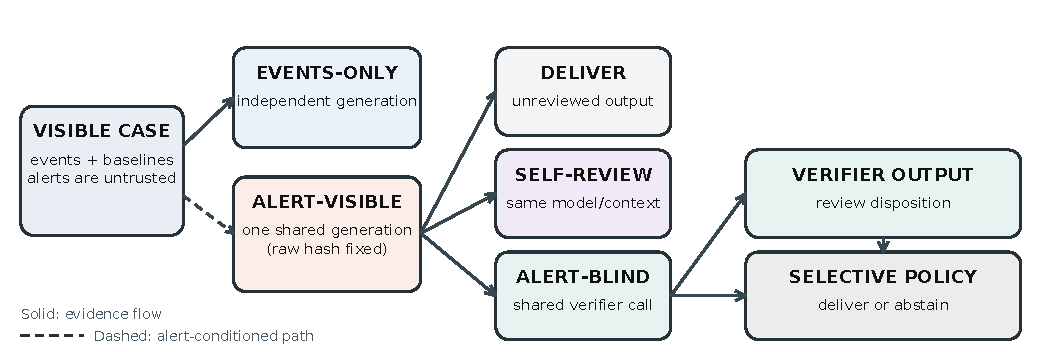
\includegraphics[width=0.96\textwidth]{figures/warrant-study-design.pdf}
\caption{Paired study design.  One alert-visible generation is reused by all
three review conditions; one alert-blind verifier response is reused by both
verifier conditions.  This makes changes after review attributable to the
policy rather than to a fresh generator sample.  Raw responses, prompts, and
hashes are retained.}
\label{fig:study-design}
\end{figure*}

\subsection{Conditions}

We evaluate five LLM conditions.  \emph{Events only} receives visible events
and baselines but no detector alert.  \emph{Events plus alerts} also receives
alerts explicitly labeled untrusted hypotheses.  \emph{Self-review} asks the
same model to inspect the shared alert-visible output for unsupported claims,
missed counterevidence, and a recommended verdict.  \emph{Generator--verifier}
uses an independently prompted, alert-blind verifier that sees the claims,
visible events, and baselines, but not detector alerts.  Finally,
\emph{verifier plus abstention} applies a deterministic policy that withholds
an output when the verifier recommends \textsc{insufficient}, the mechanical
checker finds an unwarranted decisive claim, or decisive counterevidence was
missed.

The generator receives a strict JSON schema and instructions to use direct
observations for logged facts, hypotheses for inferences, and
\textsc{insufficient} when evidence does not license a decision.  Every claim
must cite visible event identifiers.  The response is parsed exactly once;
there is no JSON repair or manual verdict recovery.  Malformed output, timeout,
and endpoint failure are retained as operational failures.

\subsection{Conservative mechanical proxy}

The deterministic evaluator resolves identifiers and checks exact or
schema-aware actor, action, object, time, and quantity matches.  Authorization
must be explicit.  Intent cannot be inferred from suspiciousness alone.
Causality requires a session, trace, request, process, or flow linkage rather
than temporal proximity.  Confirmed/observed modality requires all material
fields to be directly supported.  A decision claim inherits the warrant of its
decisive parents.

This checker is a conservative proxy, not an expert.  Its error can be
systematic: authored metadata may be clearer than production evidence, while
legitimate domain inference may be labeled insufficient.  The annotation
workflow in Section~\ref{sec:annotation} is therefore a validity requirement,
not optional decoration.

\subsection{Model and provenance policy}

The protocol targets one small local model, one stronger open-weight model,
and two frontier APIs from different providers.  The available environment
contained a 0.6B Qwen3 model, two 7.5B local Gemma-family artifacts, and a
remote OpenAI-compatible endpoint exposing only the alias
\texttt{fusion-gemma}.  Local digests, the remote endpoint hash, prompt hashes,
temperature (0.1), token limit, timestamps, latency, token counts, raw-response
path, parser state, and error state are recorded.  Because the remote revision
is not exposed and two independent frontier providers were unavailable, its
results describe one frozen deployment, not a named model family or a
cross-model capability.

Local smoke tests are retained rather than silently filtered: one 7.5B model
returned malformed output; the second produced valid JSON after a versioned
16,384-token context wrapper; Qwen3-0.6B produced a valid conservative
response.  Across all 12 development cases, Qwen3-0.6B malformed 7/12 outputs;
among valid outputs it was not competitive.  These runs establish operational
limits, not comparative accuracy.

%-------------------------------------------------------------------------------
\section{Protocol and Analysis}
\label{sec:protocol}
%-------------------------------------------------------------------------------

\subsection{Research questions and hypotheses}

The frozen protocol asks: (RQ1) how often valid citations warrant the exact
claim; (RQ2) how paired context changes affect verdict, actor, and claim
strength; (RQ3) whether systems surface counterevidence; (RQ4) whether
alert-blind verification plus abstention reduces unsafe exposure without
material recall loss; and (RQ5) what coverage, selective risk, latency, and
prevalence-adjusted precision result.

The primary hypothesis is that verifier-plus-abstention reduces unsafe claim
exposure relative to alert-conditioned generation.  Attack recall is tested
for non-inferiority with margin $\delta=0.03$.  Secondary hypotheses concern
misleading-alert flips, independent versus self-review, and decreasing
selective risk with coverage.

Protocol v1.0 originally named raw \udcr as the primary intervention outcome.
During development we recognized that a valid paired review design must reuse
the same generator response, making raw \udcr equal by construction.  Before
test inference, protocol v1.1 changed the primary safety estimand to
Eq.~\ref{eq:unsafe-exposure}; raw \udcr remains a diagnostic.  Because this
clarification followed inspection of development outcomes, we label it
outcome-aware and do not call the study preregistered.

\subsection{Repetition and independence}

Stochastic systems use three samples per case--condition pair.  The base case,
not the variant, generation, claim, or repetition, is the independent unit.
For every metric we first average repetitions and variants inside each base
case, then compute a paired intervention-minus-reference contrast.  Confidence
intervals use 10,000 complete base-case bootstrap resamples.  Exact sign tests
are descriptive at this sample size; Holm correction covers the pre-specified
secondary family.  The recall non-inferiority claim requires the lower 95\%
bound to exceed $-0.03$.

\subsection{Metrics}

We report operational validity; three-way verdict accuracy; exact verdict plus
suspect accuracy; attack recall; benign rejection; abstention and coverage;
selective exact accuracy; citation validity/completeness; raw and delivered
\udcr; unsafe exposure; decisive causal-error rate; counterevidence recall;
and paired verdict/actor flips.  At assumed incident prevalences
$\pi\in\{0.01,0.05,0.10\}$, positive predictive value is

\begin{equation}
\mathrm{PPV}(\pi)=\frac{\mathrm{TPR}\pi}
{\mathrm{TPR}\pi+\mathrm{FPR}(1-\pi)}.
\end{equation}

We do not infer workload from the benchmark prevalence.

%-------------------------------------------------------------------------------
\section{Held-Out Results}
\label{sec:results}
%-------------------------------------------------------------------------------

\subsection{Operational integrity}

The frozen test run contains \TestRecords\ records derived from
\TestBaseCases\ base cases and \TestVariants\ paired variants.  Overall
operational validity is \OperationalValidity.  Integrity verification
re-hashed each unique raw response and confirmed that alert-visible generator
hashes match across the four downstream records and verifier hashes match
across both verifier records.  No failed response was manually repaired or
excluded.

\begin{table*}[t]
\centering
\caption{Held-out results.  Unsafe exposure is unwarranted decisive claims
actually delivered per case.  Raw \udcr for the four alert-visible conditions
is identical by paired design and is not an intervention effect.}
\label{tab:main-results}
\small
\begin{tabular}{lrrrrrr}
\toprule
\textbf{Condition} & \textbf{Verdict acc.} & \textbf{Coverage} &
\textbf{Attack recall} & \textbf{Benign reject.} &
\textbf{Unsafe exposure} & \textbf{Citation valid.} \\
\midrule
Events only & \EventsAccuracy & \EventsCoverage & \EventsAttackRecall &
\EventsBenignRejection & \EventsUnsafeExposure & \AlertsCitationValidity \\
Events + alerts & \AlertsAccuracy & \AlertsCoverage & \AlertsAttackRecall &
\AlertsBenignRejection & \AlertsUnsafeExposure & \AlertsCitationValidity \\
Self-review & \SelfAccuracy & \SelfCoverage & \SelfAttackRecall & -- &
\SelfUnsafeExposure & \AlertsCitationValidity \\
Alert-blind verifier & \VerifierAccuracy & \VerifierCoverage &
\VerifierAttackRecall & -- & \VerifierUnsafeExposure & \AlertsCitationValidity \\
Verifier + abstention & \AbstainAccuracy & \AbstainCoverage &
\AbstainAttackRecall & \AbstainBenignRejection & \AbstainUnsafeExposure &
\AlertsCitationValidity \\
\bottomrule
\end{tabular}
\end{table*}

\subsection{Valid citations still carry unwarranted claims}

Alert-conditioned generation resolves \AlertsCitationValidity\ of cited event
identifiers, yet its raw \udcr is \AlertsRawUDCR\ and it surfaces
\AlertsUnsafeExposure\ unwarranted decisive claims per case.  The gap directly
answers RQ1: identifier validity is not a safety result.  Recurrent proxy
failures include causal-parent links asserted from proximity, ``observed'' or
``confirmed'' language that exceeds directly logged fields, and decisions that
inherit an insufficient parent.  Human-validated axis prevalence is reported
separately in Section~\ref{sec:annotation}; mechanical categories must not be
read as expert error rates.

\subsection{Safety is purchased with coverage}

Verifier-plus-abstention changes unsafe exposure by \UnsafeDifference\ claims
per base case (95\% CI [\UnsafeCILow,~\UnsafeCIHigh]) relative to the shared
alert-conditioned generator.  It simultaneously changes coverage by
\CoverageDifference\ [\CoverageCILow,~\CoverageCIHigh] and attack recall by
\RecallDifference\ [\RecallCILow,~\RecallCIHigh].  The lower recall bound
means the intervention \NoninferiorResult\ meet the 3-point non-inferiority
criterion.  Its delivered \udcr is \AbstainDeliveredUDCR.

This is a negative but operationally important result.  The policy can prevent
unsafe claims from reaching an analyst, but the current verifier/policy does so
by discarding too many useful investigations.  Reporting only the drop in
unsafe exposure would reward trivial refusal; reporting only selective accuracy
would hide the cases no longer covered.

\begin{figure}[t]
\centering
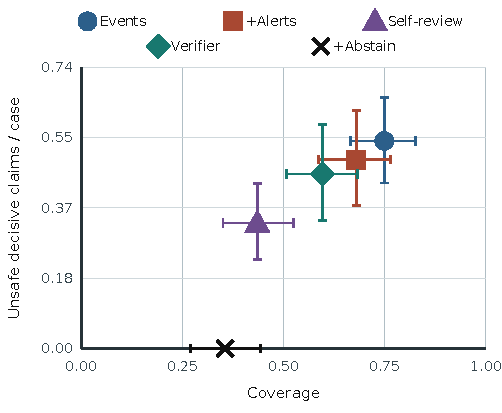
\includegraphics[width=\columnwidth]{figures/coverage-risk.pdf}
\caption{Safety--coverage operating points on held-out data.  Lower unsafe
exposure is preferable, but points farther left review fewer cases.  Error bars
are base-case cluster-bootstrap 95\% intervals.}
\label{fig:coverage-risk}
\end{figure}

\subsection{Alert context and review}

Across paired events-only and alert-visible generations, alerts change the
verdict in \AlertVerdictFlip\ of comparisons and the named actor in
\AlertActorFlip.  Variant-specific effects separate a useful alert from a
misleading actor or severity field.  Self-review does not dominate the
alert-blind verifier: it shares the generator's context and can reproduce the
same framing, while an independent verifier is less exposed to alert metadata.
Neither review approach solves the safety--coverage trade-off at the frozen
operating point.

\subsection{Baselines and prevalence}

Always-attack obtains 45\% three-way accuracy and always-benign 40\% on the 360
held-out variants.  Gradient boosting and logistic regression each obtain 85\%
three-way accuracy, while tuned rules obtain 100\%.  This ceiling is evidence
that the synthetic verdict task is transparent, not that real cloud forensics
is solved.  We therefore do not claim an LLM detection improvement over these
baselines.  Prevalence-adjusted PPV is reported only for delivered binary
decisions; abstentions are neither true nor false negatives.

%-------------------------------------------------------------------------------
\section{Human Validation}
\label{sec:annotation}
%-------------------------------------------------------------------------------

The protocol samples 400 unique material claims after deduplicating generator
responses shared across review conditions.  Sampling is deterministic and
stratified by expected verdict, generation group, claim type, and decisiveness.
Two DFIR annotators independently receive visible events, baselines, the atomic
claim, cited events, and investigation context.  They do not receive model,
condition, family, mutation, hidden label, or expected verdict.  They label
overall warrant and each semantic axis as supported, contradicted,
insufficient, or not applicable, provide a rationale, and mark materiality.
An adjudicator resolves disagreement while blinded to system identity.

The release separates a shareable blind directory from an administrative key
and hashes both.  We report raw agreement, per-label prevalence, positive
agreement, and a chance-corrected coefficient.  If expert annotation is not
completed, all warrant values in this paper remain explicitly
\emph{mechanical proxy outcomes}; H1 becomes exploratory and no claim about
true forensic-validity rates is made.  This gate prevents an authored
evaluator from validating itself.

%-------------------------------------------------------------------------------
\section{Discussion}
\label{sec:discussion}
%-------------------------------------------------------------------------------

\subsection{What the results change}

First, ``all citations resolve'' should disappear as a headline grounding
claim in evidence-bearing security systems.  It is a data-integrity check, not
a semantic safety guarantee.  Evaluation should attach to atomic claims and
include force-sensitive fields such as authorization, intent, causality, and
decision modality.

Second, alerts are not evidence merely because a SIEM produced them.  An alert
is a hypothesis with provenance and uncertainty.  Giving it to a generator can
improve focus, but it can also anchor actor and severity.  A verifier intended
to test the generator's conclusion should not receive the same untrusted
framing unless the study explicitly measures that choice.

Third, abstention must be evaluated as a selective system.  A useful operating
point reduces unsafe exposure while retaining pre-specified attack recall and
acceptable coverage.  Our frozen policy fails that joint criterion.  Future
work should calibrate claim-level confidence on disjoint data, learn axis-
specific rejection thresholds, and route only disputed material claims for
human review rather than suppressing an entire investigation.

\subsection{Deployment boundary}

The system is an analyst-assistance mechanism.  It must not autonomously accuse
a person, block an account, or initiate disciplinary action.  A delivered
claim should show cited records, missing evidence, counterevidence, alternative
hypotheses, and the reason any qualifier is warranted.  Actor and intent claims
deserve stricter review than low-level event summaries.  Raw log fields are
untrusted content, including strings that resemble instructions.

\subsection{Threats to validity}

\textbf{Construct validity.}  The mechanical evaluator encodes conservative
rules and can disagree with experts.  The synthetic generator supplies explicit
authorization and linkage fields that are often absent in practice.  Expert
annotation is therefore required for the strongest claim.

\textbf{Internal validity.}  Development data influenced prompt versions and
the v1.1 safety-estimand clarification.  We disclose both; no prompt or
evaluator change is permitted after held-out inference begins.  The generator
and reference labels share authored templates, creating correlated error.

\textbf{Statistical conclusion validity.}  There are 36 independent held-out
cases and only three nested repetitions.  Cluster intervals can be wide, family
effects are exploratory, and a failed non-inferiority test is not proof of
inferiority.  Claims and variants are never counted as independent samples.

\textbf{External validity.}  Twelve templates cannot represent production
collection gaps, organizational policies, analyst questions, or base rates.
The remote alias is revision-opaque, local small models often fail the output
contract, and two planned frontier providers are missing.  Results therefore
apply to the frozen deployment and benchmark, not ``LLMs'' in general.

\textbf{Adversarial validity.}  Passive prompt injection tests one mechanism;
it does not cover adaptive attackers, poisoned tools, compromised retrieval,
or multi-turn agent state.  Context-window truncation and provider-side safety
filters may also alter outputs.

%-------------------------------------------------------------------------------
\section{Related Work}
\label{sec:related}
%-------------------------------------------------------------------------------

\textbf{Forensic and SOC LLMs.}  Digital-forensics research warns that fluent
LLM outputs can be inaccurate, non-deterministic, and hard to admit as evidence
without validation~\cite{scanlon2023chatgpt,wickramasekara2026capabilities}.
GenDFIR combines rule-selected artifacts with retrieval-augmented timeline
reasoning~\cite{loumachi2025gendfir}; DFIR-Metric broadens knowledge and tool
evaluation~\cite{cherif2025dfirmetric}; cloud-specific work reconstructs
incidents from audit logs~\cite{alharthi2025cloud}; and CORTEX uses specialized
agents and typed tools for auditable triage~\cite{wei2025cortex}.  These systems
motivate evidence-bearing outputs.  Our distinction is the controlled
measurement of whether each cited proposition is warranted under paired
context/evidence mutations.

\textbf{Attribution and factuality.}  ALCE evaluates citation correctness and
completeness~\cite{gao2023alce}; FActScore decomposes long responses into atomic
facts~\cite{min2023factscore}; RAGAS separates context relevance,
faithfulness, and answer quality~\cite{es2024ragas}; and attributed QA studies
whether answers are supported by sources~\cite{bohnet2022attributed}.  The
closest conceptual work is FORCEBENCH, which holds evidence fixed while raising
claim force~\cite{qian2026forcebench}.  We adapt evidence-force calibration to
forensic actor, authorization, intent, causality, chronology, and decision
claims, and couple it to downstream exposure and abstention.

\textbf{Self-checking and abstention.}  SelfCheckGPT detects inconsistent
generation without an external knowledge base~\cite{manakul2023selfcheckgpt};
research-and-revise pipelines retrieve evidence to correct text
post-hoc~\cite{gao2023rarr}.  Selective classification formalizes risk--coverage
trade-offs~\cite{elyaniv2010selective,franc2023reject}, and calibration work
shows confidence need not reflect correctness~\cite{guo2017calibration}.  We
measure a review policy on a shared generator output and treat coverage loss as
a first-class outcome.

\textbf{Security context and human factors.}  Indirect prompt injection shows
that retrieved data can steer LLM-integrated applications~\cite{greshake2023not}.
SOC studies find LLM use concentrated in sensemaking rather than autonomous
high-stakes decisions~\cite{singh2025llmsoc}, while incident-response field
work reports omissions and inaccuracies in autonomous summaries
~\cite{kramer2025sir}.  These findings support the bounded analyst-assistance
posture evaluated here.

%-------------------------------------------------------------------------------
\section{Conclusion}
\label{sec:conclusion}
%-------------------------------------------------------------------------------

A real citation can support the topic of a forensic claim without supporting
its actor, intent, causal relation, or strength.  \system operationalizes this
gap with atomic claims, paired evidence mutations, an alert-blind verifier, and
selective reporting.  On the frozen held-out deployment, citation validity is
\AlertsCitationValidity while alert-conditioned generation still surfaces
\AlertsUnsafeExposure\ unwarranted decisive claims per case.  Verification plus
abstention changes exposure by \UnsafeDifference, but its attack-recall change
of \RecallDifference\ does \NoninferiorResult\ satisfy the pre-specified
non-inferiority margin.  The appropriate conclusion is not that citations make
LLM forensics safe, nor that abstention alone solves overclaiming.  Safety must
be measured at claim level and jointly with coverage; deployment must remain
analyst-supervised until independent experts validate the reference standard
and a verifier achieves a useful operating point.

\appendix

%-------------------------------------------------------------------------------
\section*{Ethical Considerations}
%-------------------------------------------------------------------------------

The benchmark is fully synthetic and contains no real users, credentials,
organizations, or routable attack infrastructure.  The work nevertheless
models a consequential use: attributing harmful activity to people.  Wrong
attribution could trigger investigation, employment action, or legal harm.
Accordingly, the evaluated system is scoped to analyst assistance and cannot
autonomously accuse, block, or discipline.  Suspect and intent fields are
treated as high-materiality claims; insufficient evidence is a valid output.
Annotators see synthetic records and inert attack strings only.  Passive prompt
injection is marked as untrusted data and is not executed.  A real deployment
would require authorization, minimization, access control, retention limits,
and documented handling for organizational logs.  The benchmark must not be
used to train punitive employee-monitoring systems or to estimate real-world
incident prevalence.

%-------------------------------------------------------------------------------
\section*{Open Science}
%-------------------------------------------------------------------------------

The anonymous artifact will include the 480-record benchmark, generation
specification and seed, data card, checksums, frozen JSON schemas and prompts,
deterministic baselines, raw model responses where provider terms permit,
response hashes and provenance manifests, parsers, the mechanical evaluator,
the blinded annotation package, analysis scripts, environment locks, tests,
and commands that regenerate every table and figure.  Endpoint secrets,
private URLs, workstation paths, and the administrative annotation key will not
appear in the reviewer artifact.  The current repository records the full
development history; an identity-scrubbed snapshot with a non-tracking URL will
be frozen for submission.  Upon acceptance, a stable public archive and an
explicit dataset license will replace the anonymous link.  Third-party models
are referenced by immutable digest when available; the revision-opaque remote
alias is disclosed rather than presented as reproducible weights.

\bibliographystyle{plain}
\bibliography{references}

\end{document}
